Voxel technology is currently an area of active research within the computer graphics community --- a Google Scholar search for the term "voxel rendering" turns up nearly 80,000 results\footnote{As of January 6\textsuperscript{th}, 2020} --- so there is no shortage of literature to draw from. 


\section{Technologies}
\subsection{Programming Language}
The choice of programming language and environment has an enormous impact on the project's life cycle. Since this project is designed for use in interactive video game engines, a language supporting compilation to native code was mandatory. Additionally, as this project will need to carefully orchestrate data flow between the CPU and GPU, support for control over low-level implementation details such as data alignment and memory layout was also required.

With these concerns in mind, I evaluated three programming languages: C, C++ and Rust. Though Rust boasts some very attractive features such as guaranteed memory safety and a powerful type system, it is still a very new programming language, with a very small userbase in the commercial game programming community. C++ is a strong candidate, however it is generally more difficult to integrate a C++ class library with other languages than a pure C function library because many languages (Lua, for example) expect foreign code to conform to a C API. C has the advantage of simplicity, but I would prefer to avail of the better type-checking built into most C++ compilers for this project.

After evaluating each of the above programming languages, I have chosen to implement this project in C++, but exporting a C API. This means that the library code should be usable from other programming languages which expect a C API, while still allowing me to take advantage of C++'s more ergonomic features, such as raw string literals and operator overloading. 

\subsection{Graphics API}
An essential component of any high-performance graphics application is the API used to issue GPU instructions. This is an important decision to make for the project as the code required to perform some operation may look considerably different between separate graphics APIs, so the choice of API has a large impact on the final codebase.

Excluding manufacturer-specific options, there are four main graphics APIs used to write high-performance GPU code today:

\begin{itemize}
    \item OpenGL, a cross-platform and community-driven API originally developed by Silicon Graphics Inc. and now managed by the Khronos Group. Modern versions of the OpenGL API support advanced low-level techniques such as compute shaders and shader storage buffers required to render large amounts of voxels on the GPU. In OpenGL the graphics card may be programmed using GLSL, a high level programming language with special support for computer graphics operations.
    
    \item Direct3D (D3D), a proprietary graphics API developed by Microsoft. Part of the DirectX family of SDKs, D3D offers a high-level API with features roughly comparable to OpenGL along with its own GPU programming language, HLSL. As it is controlled entirely by Microsoft, Direct3D is limited to the Windows and XBox platforms.
    
    \item Vulkan, a cross-platform API recently introduced by the Khronos group in 2016 as an alternative to OpenGL. The primary motivation for introducing a new API was to provide application programmers more fine-grained control over the GPU's actions, and to take better advantage of the massively parallel nature of GPU systems . Vulkan allows for extremely granular control over an application's resource usage, though this requires significantly more management code to be written. Vulkan shaders are compiled offline into an assembly-like intermediate representation called SPIR-V. As such, Vulkan shaders may be written in either GLSL or HLSL but an appropriate compiler is needed to transform the shader source into SPIR-V assembly.
    
    \item Metal, a proprietary API developed by Apple Inc. Metal was introduced in 2014 for much the same reasons as Vulkan, and is quite similar in design. Metal uses its own shading language called "the Metal shading language".
\end{itemize}

In the above options, there is a clear distinction between OpenGL and Direct3D, and Vulkan and Metal. These latter two APIs were designed much later than OpenGL and Direct3D, and more closely resemble how modern GPUs function. As such, they can potentially provide much greater performance and control over GPU resources, but at the cost of code complexity  \autocite{wyman2015vulkan}.

When selecting a graphics API for use in this project, I based my choice primarily on how familiar I was already with each API. Since I was already familiar with modern OpenGL programming, and OpenGL code can run on more platforms than Direct3D code, I chose to use OpenGL as the graphics API for this project. Although I would have liked to explore the newer Vulkan API, I do not have easy access to hardware compatible with Vulkan.

\subsection{Tools}\label{sec:tools}
Since I was developing primarily on the Windows operating system, I chose to use Microsoft WinDBG as my debugger. WinDBG is a source-level debugger which supports custom scripting, disassembly and time-travel debugging.

Traditional debuggers can only examine code running on the CPU. As this project relies heavily on GPU code to render the voxel scene, a tool capable of debugging GPU code was required. Graphics debuggers are more closely tied to the underlying hardware than CPU debuggers; NVidia and ATI both offer products which only work on the respective manufacturer's hardware. Since I own a NVidia graphics card, I chose NVidia's Nsight Graphics as my graphics debugger.

\begin{figure}[h]
    \centering
    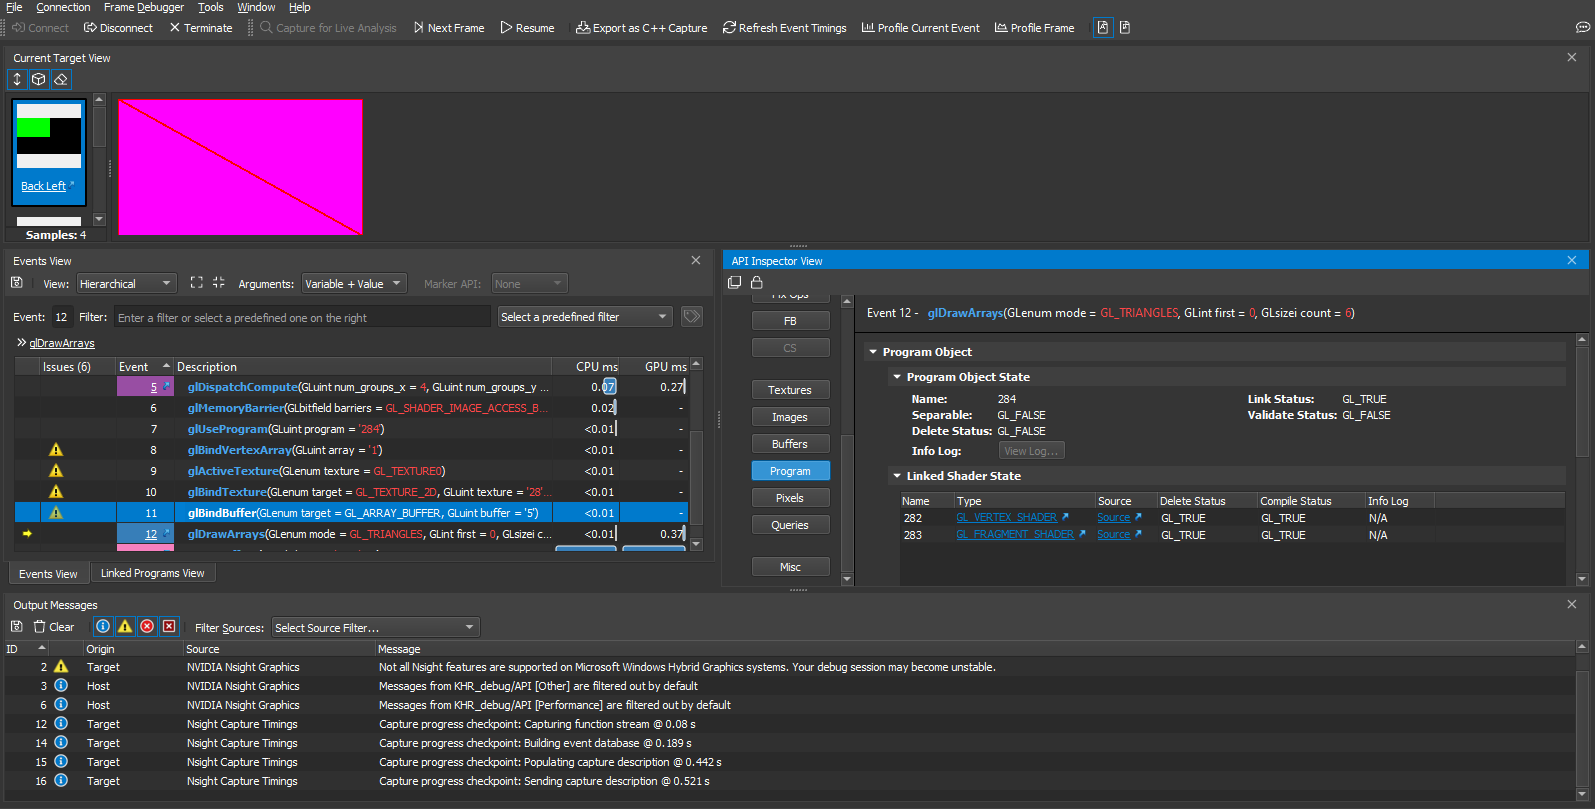
\includegraphics[width=400px]{graphics/nsight_screenshot.png}
    \caption{A screenshot of the viewer application running under Nsight Graphics}
    \label{fig:nsight_screenshot}
\end{figure}

To streamline development across multiple machines, and to have safe, reliable code storage I chose Git as my version control system, with the project being hosted on GitLab.com. 

\section{Mathematics}
Since one of my primary goals for this project is to become more proficient with 3D game engine programming, I have decided to write the entirety of the mathematics code myself. Having some previous experience in this task already, I began by porting several maths utilities I had previously written in C++ to this project. This ad-hoc math library contains some very simple vector operations (dot product, cross product, normalisation formula), some matrix operations (vector-matrix product, matrix-matrix product) and some miscellaneous functions specifically related to graphics programming such as the perspective projection formula.

My primary reference for mathematics was Lengyel's \textit{Foundations of Game Engine Development, Volume 1: Mathematics} \autocite{lengyel2016math}. I also relied heavily on my Computer Graphics II course notes for developing the perspective projection code \autocite{healy2019perspective}.

I also utilised quaternions for handling camera rotations in the prototype renderer, and I plan to do the same in the final viewer application. A quaternion can encode a rotation more efficiently than a matrix because it only requires four floating-point numbers to store the rotation as opposed to the sixteen required by a matrix. I used Van Verth's excellent overview to gain an understanding of the theory behind quaternion rotation, in particular the quaternion multiplication formula and how to rotate a vector by a quaternion \autocite{van2013understanding}.

\section{Data Storage}
When starting this project, I knew I would require a data structure capable of storing massive amounts of voxel data in an efficient form. Initially, I considered classical pointer-based Octrees. Octrees are a type of hierarchical data structure used to efficiently represent 3D space by discarding large empty regions. They were first introduced by Meagher in 1980 \autocite{meagher1980octree}. In their most basic form, octrees use eight child-pointers to link parent and child nodes together. Laine and Karras improved on this design by encoding child data inside parent nodes; their design uses eight bit masks to determine whether or not a particular node has children, and if its children are leaf nodes. This removes the need to store leaf nodes at all.


\section{Rendering Methods}
Techniques available for rendering voxel data can be split into two broad categories: polygon-based methods and volumetric methods. Polygon-based methods represent the scene to be rendered as a collection of voxels in memory, but convert it to a polygon mesh before rendering. Once the scene has been converted into a polygon mesh, it can then be rendered in the same way as any other polygon. There are many algorithms available for transforming a field of voxels into a polygon mesh, one of which I initially planned to use in this project: Marching Cubes \autocite{lorensen1987marching}.

Though I considered using polygon rendering for this project, I decided not to proceed with it because the rendered polygon meshes will inherit all of the limitations of existing polygon geometry while simultaneously incurring the memory overhead of voxel storage. Using polygon rendering would require re-creating the polygon mesh of a voxel object every time it was changed. Instead I chose to use \textit{ray-casting} for this project --- a volumetric rendering approach which operates by shooting a ray into the voxel scene and examining all voxels intersected by the ray. The output image is produced by casting a ray for each pixel on the screen.

Laine and Karras introduce a voxel ray-casting algorithm in their \textit{Efficient sparse voxel octrees} paper \autocite{laine2010efficient}. I have based my GLSL code on their approach.

\subsection{OpenGL Compute Shaders}
Since ray-casting is a highly parallelisable problem, it is well-suited to GPUs. I chose to use OpenGL compute shaders to perform the ray-casting due to the fact that I was already familiar with the GLSL programming language. To learn the specifics of compute shader programming, I began by reading an excellent overview by Mike Bailey \autocite{bailey2014}. I also used the official OpenGL reference pages to look up specific API details while programming \autocite{gldocs}.

To set up a proper rendering pipeline, I used the approach detailed by Burjack in the online tutorial article \textit{Ray tracing with OpenGL Compute Shaders (Part I)} \autocite{burjack2017}. This involved first creating an OpenGL image object to represent the output image. For each square "tile" of some small number of pixels, a compute shader is executed to fire a ray into the scene and perform the actual ray-casting computations. If the ray intersects voxel geometry, the tile is filled with colour. The final image is produced by executing the same compute shader many times for all of the output image's constituent tiles. Finally, this image is rendered onto a quadrilateral polygon mesh to produce the scene render.

\subsection{Ray-Box Intersection}
A crucial component of any ray-casting engine is how to determine when a ray intersects a voxel. I began by implementing Tavian Barnes' intersection algorithm \autocite{barnes2011} in GLSL. Some time later, I came across another version of the same algorithm by Majercik et al. \autocite{majercik2018ray} which uses GLSL's built-in vector math functions to more concisely express the same operation.

\section{Polygon Renderer Prototype}\label{sec:poly_renderer_research}
The earliest development work on this project began with a prototype voxel renderer which transformed voxel data into polygon meshes using Lorensen and Cline's Marching Cubes algorithm. This prototype allowed me to get familiar with low-level OpenGL programming.

This prototype showcases one of the core strengths of voxel-based technology: the ability to automatically generate geometry. Figure \ref{fig:polygon_renderer_sphere} shows a sphere built entirely out of voxels. This sphere was generated by filling all voxels which satisfied the following implicit surface function:
$$
x^2 + y^2 + z^2 - r^2 = 0
$$

The remaining voxels are considered "air" or empty.


\begin{figure}[ht]
    \centering
    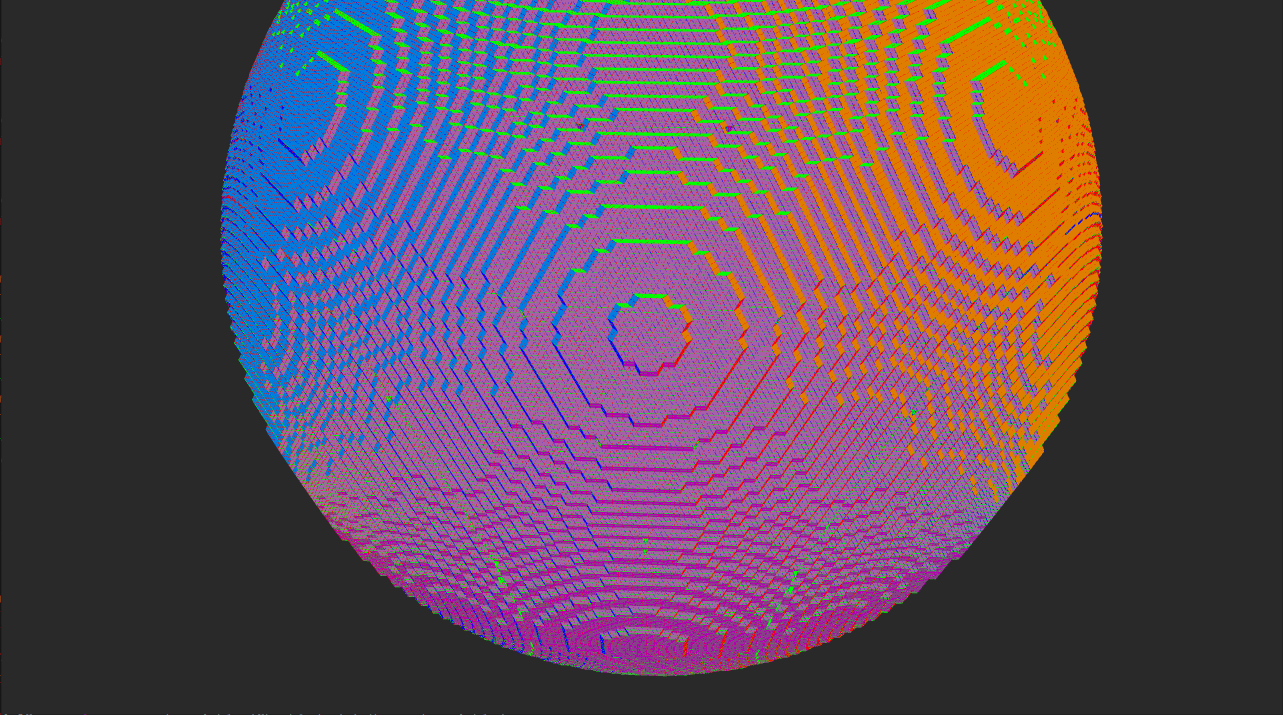
\includegraphics[width=400px]{graphics/prototype_sphere.png}
    \caption{A screenshot from the prototype polygon renderer showing a sphere built from voxels}
    \label{fig:polygon_renderer_sphere}
\end{figure}

This prototype stored all voxel data in a simple array, with individual voxels addressed by their 3D coordinates. Albeit simple, this approach was, fundamentally, a poor choice for the final implementation because of its poor scalability. Storing all of the voxel data in a single flat array places a hard limit on the number of voxels available to represent the scene.
